% Created 2026-04-22 Wed 22:23
% Intended LaTeX compiler: lualatex
\DocumentMetadata{lang = en, pdfversion = 2.0, pdfstandard = ua-2, pdfstandard = a-4, testphase = {phase-III, title, table, math, firstaid}}
\documentclass[11pt]{article}
\usepackage{amsmath}
\usepackage{fontspec}
\usepackage{graphicx}
\usepackage{longtable}
\usepackage{wrapfig}
\usepackage{rotating}
\usepackage[normalem]{ulem}
\usepackage{capt-of}
\usepackage{hyperref}
\usepackage[margin=1in]{geometry}
\usepackage{fontspec}
\usepackage{verbatim, multicol, tabularx,}
\usepackage{amsmath, amsthm, amssymb, stmaryrd, latexsym, bm, listings, qtree}
\usepackage{framed}
\usepackage{xcolor,colortbl}
\usepackage{media9}
\usepackage[export]{adjustbox}
\usepackage{algorithm}
\usepackage[noend]{algpseudocode}
\usepackage{tikz,pgfplots}
\usetikzlibrary{shapes.geometric}
\let\oldquote=\quote
\let\endoldquote=\endquote
\colorlet{shadecolor}{cyan!15}
\renewenvironment{quote}{\begin{shaded*}\begin{oldquote}}{\end{oldquote}\end{shaded*}}
% From https://tex.stackexchange.com/questions/7032/good-way-to-make-textcircled-numbers
\newcommand*\circled[1]{\tikz[baseline=(char.base)]{\node[shape=circle,draw,inner sep=2pt] (char) {#1};}}
\DeclareMathOperator*{\argmin}{arg\!min}
\DeclareMathOperator*{\argmax}{arg\!max}
\lstset{frame=tb, aboveskip=1mm, belowskip=0mm, showstringspaces=false, columns=flexible, basicstyle={\scriptsize\ttfamily}, numbers=left, frame=single, breaklines=true, breakatwhitespace=true}
\hypersetup{colorlinks=true,urlcolor=blue}
\usepackage{polyglossia}
\setdefaultlanguage[variant=US]{english}
\author{Christopher Simpkins}
\date{Kennesaw State University}
\title{Artificial Intelligence\\\medskip
\large Multiagent Systems (AIMA 18.1, MAS 1-2)}
\hypersetup{
 pdfauthor={Christopher Simpkins},
 pdftitle={Artificial Intelligence},
 pdfkeywords={},
 pdfsubject={Artificial Intelligence Multiagent Systems (AIMA 18.1, MAS 1-2)},
 pdfcreator={Emacs 30.2 (Org mode 9.7.11)}, 
 pdflang={English}}
\begin{document}

\maketitle
\section{Multiagent Systems}
\label{sec:orgada8043}


Dealing with multiagent environments:

\begin{itemize}
\item Single agent with other agents considered part of the environment
\item Multiple actors, but one decision maker controlling all actors
\item Multiple actors, each of which makes its own decisions
\end{itemize}






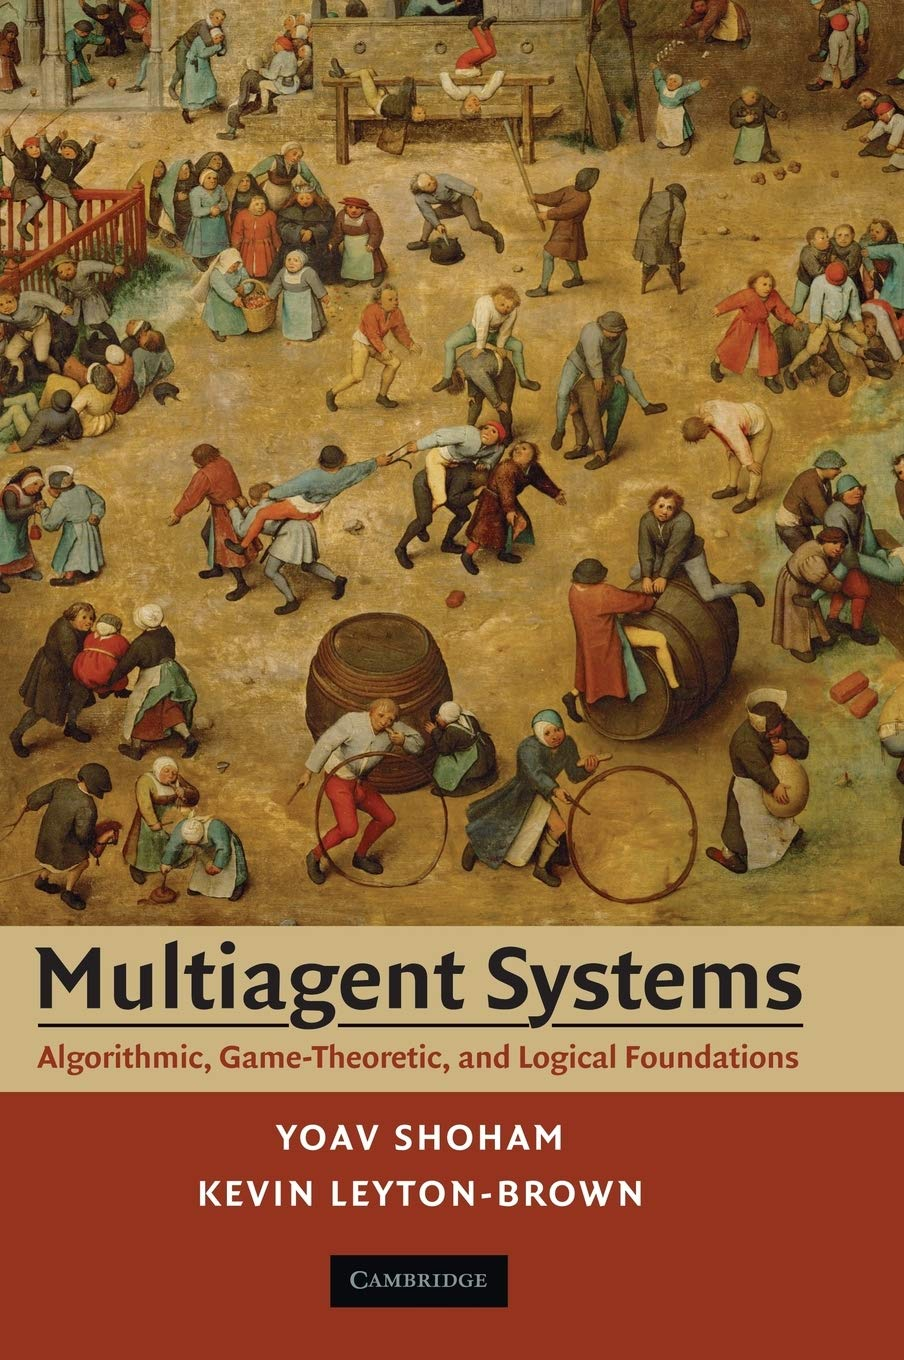
\includegraphics[alt={mas book},height=2.0in]{mas-book.jpg}



MAS: \url{https://www.masfoundations.org/}






\includegraphics[alt={marl book},height=2.0in]{marl-book.jpg}



MARL: \url{https://www.marl-book.com/}
\section{Multiagent Environments}
\label{sec:org9d6c4c4}

Dealing with multiagent environments:

\begin{itemize}
\item Single agent with other agents considered part of the environment
\item Multiple actors, but one decision maker controlling all actors
\item Multiple actors, each of which makes its own decisions
\end{itemize}
\section{One Decsion Maker}
\label{sec:org0627bfd}

Rests on \textbf{benevolent agent assumption}: agents will do what they are told.

Action synchronization:

\begin{itemize}
\item Sumultaneous/joint actions
\item Mutually exclusive actions executed at different times
\item Sequential actions \(A\) before \(B\) when \(A\)'s postconditions are \(B\)'s preconditions
\end{itemize}

Architectures:

\begin{itemize}
\item \textbf{Multieffector planning}: multiple concurrently acting effectors
\item \textbf{Multibody planning}: physically decoupled effectors

\begin{itemize}
\item Centralized planning: sensor information from each body is pooled
\item Decentralized planning: plan execution partially or fully decoupled, explicit communication to share information when possible (e.g., back in comms range)
\end{itemize}
\end{itemize}
\section{Multiple Decision Makers}
\label{sec:org0f4134c}

All agents, a.k.a. \textbf{counterparts}, make decisions.  Two categories:

\begin{enumerate}
\item Agents have a \textbf{common goal}.

\begin{itemize}
\item Agents \textbf{coordinate} to accomplish common goal, e.g., workers in a company, players on a team
\end{itemize}

\item Agents have differeent goals.

\begin{itemize}
\item Goals may be unrelated, diametrically opposed (e.g., zer-sum games), or anythin in between.
\end{itemize}
\end{enumerate}
\section{Game Theory}
\label{sec:org22b3c89}

Multiple decision makers pursuing their own preferences.

\begin{itemize}
\item An agent must take into account preferences of other agents.
\item These other agents also take into account preferences of other agents, and so on.
\end{itemize}

\textbf{Game theory}: the theory of \textbf{strategic decision making}.

\begin{itemize}
\item \textbf{Strategic} because decisions must take into account how other players act.
\item Strategic aspect distinguishes game theory from decision theory.
\end{itemize}

Just as decision theory provides the theoretical foundation for single-agent decision making, game theory provides the theoretical foundation for multiagent decision making.
\section{Game Theory in AI}
\label{sec:orgcd38651}

In AI, game theory can be used in two main ways:

\begin{enumerate}
\item \textbf{Agent design}: analyzing decisions in multiagent environments.

\begin{itemize}
\item Enumerate possible decisions
\item Compute expected utility of each decision
\end{itemize}

\item \textbf{Mechanism design}: deisgn multiagent environment in such a way that when agents act selfishly to maximize utility, it has the effect of maximizing some collective good.

\begin{itemize}
\item Example: protocols for Internet routers
\item Example: criminal legal system
\end{itemize}
\end{enumerate}
\section{Cooperative vs Noncooperative Games}
\label{sec:org5db629b}

Two broad categories of game models:

\begin{enumerate}
\item Cooperative games:

\begin{itemize}
\item Binding agreement between agents ensuring cooperation.
\end{itemize}

\item Noncooperative games:

\begin{itemize}
\item Not necessarily competitive.
\item Simply means no binding agreement to cooperate.
\end{itemize}
\end{enumerate}

Often mix models:

\begin{itemize}
\item Package company: centralized planning for routes and trucks, decentralized execution via autonomous decisions of drivers and pilots responsing individually to real-time conditions.
\item Company: individual \textbf{incentives} for employees designed to bring their behavior into alignment with company's goals.
\end{itemize}
\section{Multiagent Planning}
\label{sec:org07589b6}

Use generic term \textbf{actor} for effectors, bodies and agents.  Need to define:

\begin{itemize}
\item transition models
\item correct plans
\item planning algorithms
\end{itemize}

Agents must take into account the way in which their own actions interact with the actions of other agents.

\begin{itemize}
\item Example: Agent \(A\)'s action might clobber the precoditions of the action Agent \(B\) planned to execute.
\end{itemize}
\section{Concurrency Models}
\label{sec:org59c5d5e}

Three approaches to dealing with concurrency:

\begin{enumerate}
\item \textbf{Interleaved execution}.  Given Agents \(A\) and \(B\) with plans \([a_1, a_2]\) and \([b_1, b_2]\) there are six ways to execute them concurrently:

```\{=latex\}
\begin{align*}
[a_1,a_2,b_1,b_2]\\
[b_1,b_2,a_1,a_2]\\
[a_1,b_1,a_2,b_2]\\
[b_1,a_1,b_2,a_2]\\
[a_1,b_1,b_2,a_2]\\
[b_1,a_1,a_2,b_2]
\end{align*}
```

\begin{itemize}
\item Plans must be correct with respect to all possible interleavings.
\item Popular in OS concurrency on single CPU.
\item Does not model true concurrency, i.e., simultaneous action.
\item Number of sequences grows exponentially with numbers of agents and actions.
\end{itemize}

\item \textbf{True concurrency}: leave plans \textbf{partially ordered} and don't create a fully serialized ordering.

\item \textbf{Synchronization}: global clock, each action takes one time step, joint actions execute simultaneously, no-ops in case "waiting" is needed.
\end{enumerate}
\section{Multiagent Transition Models}
\label{sec:org3201feb}

Deterministic single-agent case: `RESULT(s, a)` with \(b\) choices for the action.

Multiagent case: with \(n\) actors, joint action \(\langle a_1, \dots, a_n \rangle\) where \(a_i\) is actoin taken by  \$i\$th actor.

\begin{itemize}
\item Must describe transition model for \(b^n\) joint actions.
\item Joint planning problem with branching factor of \(b^n\).
\end{itemize}

Standard solution: pretend problems are decoupled and fix the interactions as they arise, i.e., writing action schemas as if actors acted independently.  Let's see how this works with an example \ldots{}
\section{Example: Doubles Tennis Planning}
\label{sec:org9d5b628}





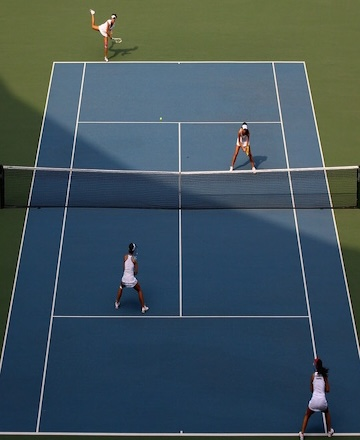
\includegraphics[alt={doubles tennis},width=0.75\linewidth]{doubles-tennis.jpg}







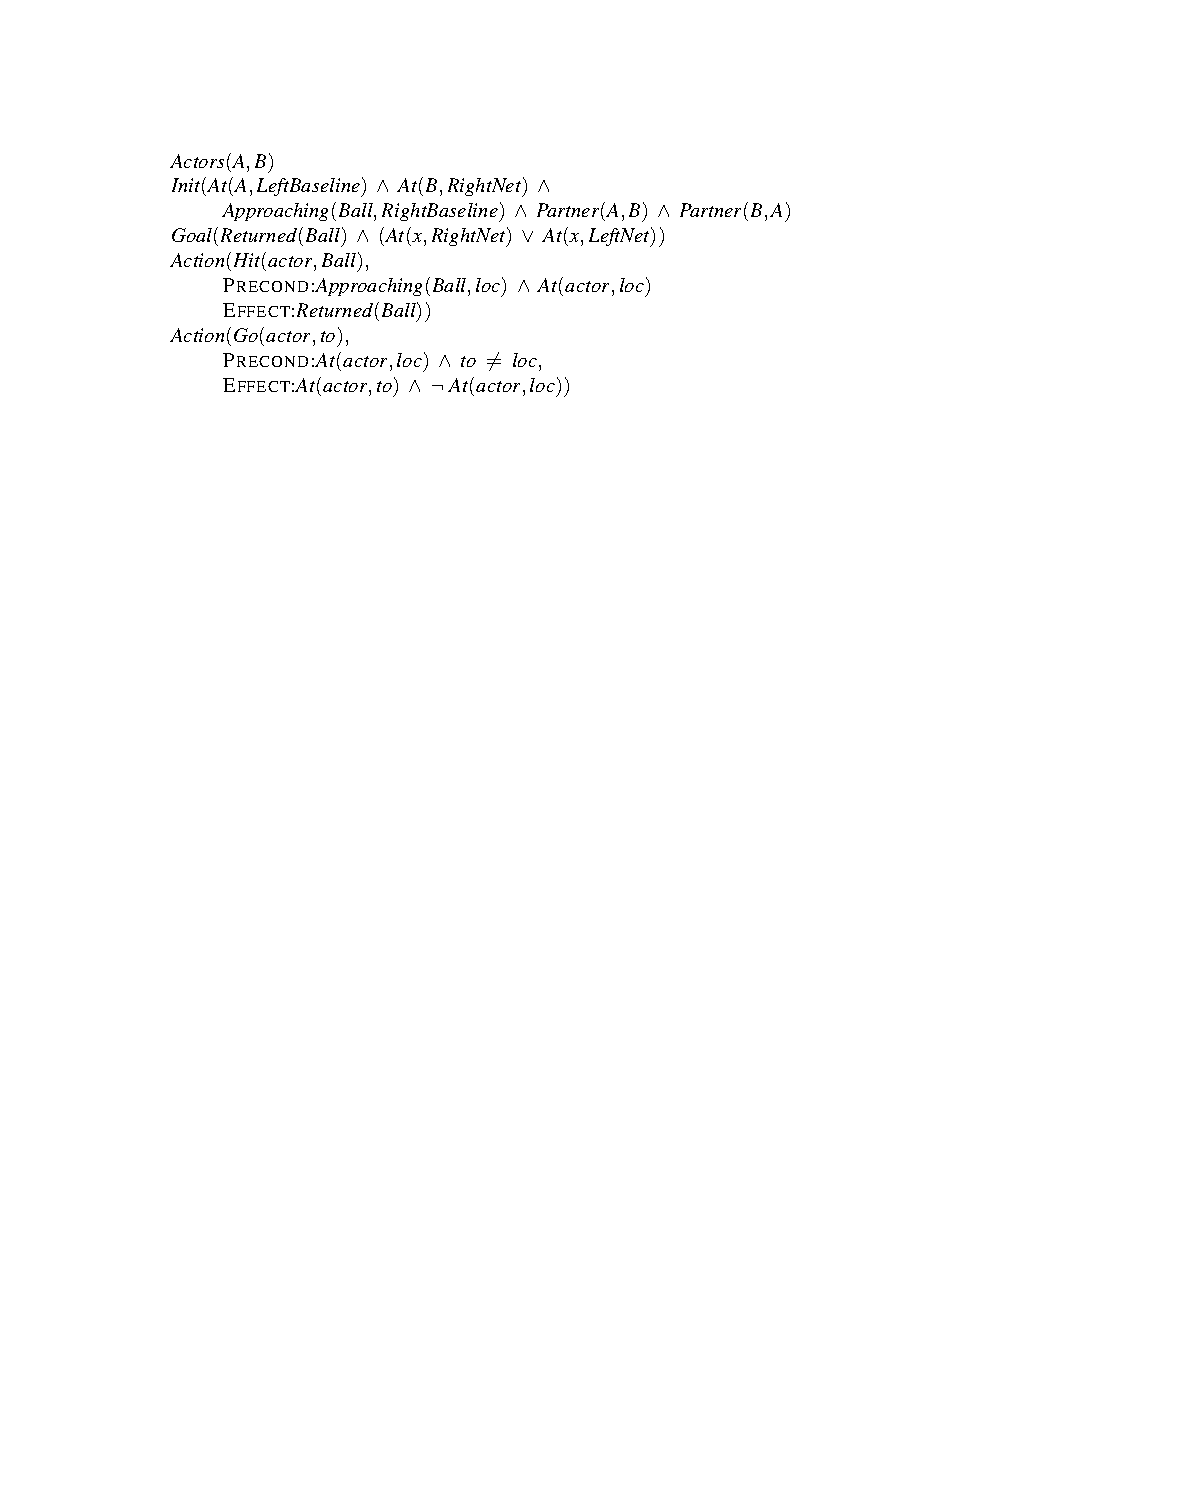
\includegraphics[alt={aima fig 18_01 doubles tennis problem},width=0.75\linewidth]{aima-fig-18_01-doubles-tennis-problem.pdf}



Here's a 2-step \textbf{joint plan} that works:

\begin{align*}
\text{PLAN 1}: &A : [Go(A,RightBaseline),Hit(A,Ball)] \\
               &B : [NoOp(B),NoOp(B)].
\end{align*}
\section{Concurrent Action Constraints}
\label{sec:orgdc50546}


What if both players try to \(Hit\) at the same time?  Add a \textbf{concurrent action constraint} to prevent:

\vspace{-.25in}
\begin{align*}
& Action(Hit(actor, Ball),\\
& \hspace{.1in} \text{CONCURRENT:} \forall b, b \neq Actor \implies \neg Hit(b, Ball)\\
& \hspace{.1in} \text{PRECOND:} Approaching(Ball, loc) \land At(actor, loc) \\
& \hspace{.1in} \text{EFFECT:} Returned(Ball))
\end{align*}
\vspace{-.25in}

Some tasks require concurrent action, e.g., carrying a large cooler:

\vspace{-.25in}
\begin{align*}
& Action(Carry(actor, cooler, here, there),\\
& \hspace{.1in} \text{CONCURRENT:} \exists b, b \neq Actor \land Carry(b, cooler, here, there) \\
& \hspace{.1in} \text{PRECOND:} At(actor, here) \land At(cooler, here) \land Cooler(cooler) \\
& \hspace{.1in} \text{EFFECT:} At(actor, there) \land At(cooler, there) \land \neg At(actor, here) \land \neg At(cooler, here)
\end{align*}
\vspace{-.25in}
\section{Cooperation and Coordination}
\label{sec:org7567e99}

There can be multiple joint plans that acheive the goal:




\begin{align*}
\text{PLAN 1}: &A : [Go(A,RightBaseline),Hit(A,Ball)] \\
               &B : [NoOp(B),NoOp(B)].
\end{align*}




\begin{align*}
\text{PLAN 2}: &A : [Go(A,LeftNet),NoOp(A)] \\
               &B : [Go(B, RightBaseline), Hit(B, Ball)]
\end{align*}




If both agents choose Plan 1 or 2, goal is acheived.  If one agent chooses 1 and other chooses 2, goal is not acheived.  How to coordinate?

\begin{itemize}
\item \textbf{Convention}: any constraint on selection of joint plans.

\begin{itemize}
\item Example: "stick to your side of the court."
\item Widespread conventions are sometimes called \textbf{social laws}.
\end{itemize}

\item \textbf{Communication}

\begin{itemize}
\item Example: shout "Mine!" or "Yours!"
\item Can be implicit, based on observation -- \textbf{plan recognition}.
\end{itemize}
\end{itemize}
\section{Games with a Single Move: Normal Form Games}
\label{sec:org4338ee8}

All players take action that are chosen simultaneously with no knowledge of other players' choices and the result of the game is based on the profile of actions that are selected in this way.

\textbf{Normal form game} defined by:

\begin{itemize}
\item A finite set \(N\) of \(n\) \textbf{players} (agents) making decisions. Two-player games most studied, but games for \(n > 2\) also common.

\item \textbf{Actions} \(A = A_i \times \cdots \times A_n\), where \(A_i\) is a finite set of actions available to player \(i\).  Each vector \(a = (a_i, \dots, a_n)\) is called an \textbf{action profile} or a \textbf{strategy}.

\item \textbf{Payoff function} \(u = (u_i, \dots, u_n)\) where \(u_i \colon A \mapsto \mathbb{R}\) is the utility/payoff function for player \(i\). Here we assume outcomes \(O\) are completely determined by \(A\).

\begin{itemize}
\item For two-player games, payoff function can be represented by a matrix in which there is a row for each possible action of one player, and a column for each possible choice of the other player: a chosen row and a chosen column define a matrix cell, which is labeled with the payoff for the relevant player. In the two- player case, it is conventional to combine the two matrices into a single \textbf{payoff matrix}, in which each cell is labeled with payoffs for both players.
\end{itemize}
\end{itemize}
\section{Example: Two-Finger Morra}
\label{sec:org3a92b74}

Here is the payoff matrix for \textbf{two-finger Morra}, a game in which each player displays one or two fingers.


\begin{tabular}{|c|c|c|}\hline
       & O: one         & O: two         \\\hline
E: one & E = +2, O = -2 & E = -3, O = +3 \\\hline
E: two & E = -3, O = +3 & E = +4, O = -4 \\\hline
\end{tabular}


\begin{itemize}
\item \(E\) is the \textbf{row player}, \(O\) is the \textbf{column player}.
\item Each cell shows the payoffs given the players' actions.
\end{itemize}
\section{Solution Concepts}
\label{sec:org9c1f080}

A \textbf{solution concept} is a way of choosing actions that take other players' actions into account.  Some important terminology:

\begin{itemize}
\item \textbf{Strategy}: like a policy, but we must account for the actions of the other players.

\item \textbf{Pure strategy}: a deterministic strategy/policy.  For a single-move game, a single action.

\item \textbf{Mixed strategy}: a randomized policy.  The mixed strategy that chooses action \(a\) with probability \(p\) and action \(b\) otherwise is written \([p:a;(1 - p):b]\).

\begin{itemize}
\item Two-finger Morra example: \([0.5:one;0.5:two]\)
\end{itemize}

\item \textbf{Strategy profile}: an assignment of a strategy to each player.

\item \textbf{Outcome}: a numeric value for each player.  For mixed strategies, this is expected utility.
\end{itemize}

Solution concepts define rationality in games.
\section{The Prisoner's Dilemma[\textsuperscript{PD}]}
\label{sec:org0f4bac8}

Two prisoners, \(A\) and \(B\), suspected of committing a crime together are taken to separate interrogation rooms, and each can either "confess" to the crime (a.k.a. "cooperate") or "deny" it (a.k.a. "defect").

\begin{itemize}
\item If both prisoners confess/cooperate, each gets a 1-year sentence.
\item If both prisoners deny/defect, each gets a 3-year sentence
\item If one player denies and the other confesses, the the confessor ("sucker"/cooperator) gets 5 years and the denier (defector) gets 0 years.
\end{itemize}

The game can be summarized in the following payoff matrix (row player's payoff is listed first):


\begin{tabular}{|c|c|c|}\hline
       & B: c         & B: d         \\\hline
A: c & -1, -1 & -5, 0 \\\hline
A: d & 0, -5  & -3, -3 \\\hline
\end{tabular}


The dillemma: should they confess or deny?

{[}\textsuperscript{PD}]: We adopt the more common notation found, e.g., in \url{https://www.marl-book.com/}, \url{https://www.masfoundations.org/}, and \url{https://www.amazon.com/Evolution-Cooperation-Robert-Axelrod/dp/1541606841/}
\section{The TCP Game[\textsuperscript{TCP}]}
\label{sec:org40d73aa}

Internet traffic is governed by the TCP protocol. One feature of TCP is the \textbf{backoff} mechanism; if your data rates cause congestion, back off until congestion subsides.

Consider a world of two TCP users, \(A\) and \(B\).

\begin{itemize}
\item If both users use a corect TCP implementation, \(c\), each gets a 1 ms packet delays.
\item If both users use a defective TCP implementation, \(d\), each gets a 3 ms packet delays.
\item If one user uses a correct implmentation and the other a defective one, the correct user (or "sucker") gets 5 ms packet delays and the other gets 0 ms delays.
\end{itemize}


\begin{tabular}{|c|c|c|}\hline
       & B: c         & B: d         \\\hline
A: c & -1, -1 & -5, 0 \\\hline
A: d & 0, -5  & -3, -3 \\\hline
\end{tabular}


The Prisoner's dilemma is widely applicable.  In general:


\begin{tabular}{|c|c|c|}\hline
       & C         & D        \\\hline
C & a, a & b, c \\\hline
D & c, b & d, d  \\\hline
\end{tabular}


with \(c > a > d > b\).  Adding \(a > \frac{b+c}{2}\) guarantees that \((C, C)\) maximizes the sum of the agents' utilities/payoffs.

{[}\textsuperscript{TCP}]: \url{https://www.masfoundations.org/} Section 3.2.1-3.2.3
\section{Dominant Strategies and Equilibria}
\label{sec:orgeeeb801}




Consider \(A\)'s response when \(B\)'s strategy is \(c\):


\begin{tabular}{|c|c|c|}\hline
       & B: c         & B: d                 \\\hline
A: c & \cellcolor{lightgray} -1, -1 &  -5, 0 \\\hline
A: d & \cellcolor{lightgray} 0, -5   & -3, -3 \\\hline
\end{tabular}


\(A\)'s highest payoff is with \(d\).

How about when \(B\)'s strategy is \(d\):


\begin{tabular}{|c|c|c|}\hline
       & B: c         & B: d                 \\\hline
A: c & -1, -1  & \cellcolor{lightgray} -5, 0  \\\hline
A: d & 0, -5   & \cellcolor{lightgray} -3, -3 \\\hline
\end{tabular}


Again, \(A\)'s highest payoff is with \(d\).  No matter what \(B\) does, \(A\)'s \textbf{best response} is \(d\).  So \(d\) is a \textbf{dominant strategy} for \(A\) -- \(d\) acheives the highest payoff in response to every possible action of \(B\).




Consider \(B\)'s response when \(A\)'s strategy is \(c\):


\begin{tabular}{|c|c|c|}\hline
       & B: c         & B: d                                      \\\hline
A: c & \cellcolor{lightgray} -1, -1  & \cellcolor{lightgray} -5, 0 \\\hline
A: d & 0, -5                         & -3, -3                      \\\hline
\end{tabular}


\(B\)'s highest payoff is with \(d\).

How about when \(A\)'s strategy is \(d\):


\begin{tabular}{|c|c|c|}\hline
       & B: c         & B: d                                      \\\hline
A: c & -1, -1                      & -5, 0                         \\\hline
A: d & \cellcolor{lightgray} 0, -5 & \cellcolor{lightgray}-3, -3   \\\hline
\end{tabular}


Again, \(B\)'s highest payoff is with \(d\).  No matter what \(A\) does, \(B\)'s \textbf{best response} is \(d\).  So the \textbf{dominant strategy} for \(B\) is also \(d\).




When all players choose a dominant strategy, the result is a \textbf{dominant strategy equilibrium}.

\begin{itemize}
\item An \textbf{equilibrium} is a state where no player has an incentive to change their action.
\end{itemize}

Choosing a dominant strategy is \textbf{rational}.  But notice that the payoff under strategy profile \((d, d)\) is \([-3, -3]\) whereas the payoff for strategy profile \((c, c)\) is \([-1, -1]\).
\section{Optimal Strategies and Social Welfare}
\label{sec:org295f081}

An \textbf{optimal strategy} for an agent optimizes the payoff/utility for that agent.  From the standpoint of \textbf{social welfare} we want to optimize the utility of all agents.

\begin{itemize}
\item Strategy profile \(s\) \textbf{Pareto dominates} strategy profile \(s'\) if for all \(i \in N\), \(u_i(s) \ge u_i(s')\), and there exists some \(j \in N\) for which \(u_j(s) > u_j(s')\).
\end{itemize}
\end{definition}

\begin{itemize}
\item Strategy profile \(s\) is \textbf{Pareto optimal}, or \textbf{strictly Pareto efficient}, if there does not exist another strategy profile \(s' \in S\) that Pareto dominates \(s\).

\item An outcome is \textbf{Pareto optimal} if there is no other outcome that would make one player better off without making someone else worse off. If you choose an outcome that is not Pareto optimal, then it wastes utility in the sense that you could have given more utility to at least one agent, without taking any from other agents.
\end{itemize}

Utilitarian social welfare is a measure of how good an outcome is in the aggregate.  Two difficulties:

\begin{itemize}
\item Considers the sum but not the distribution of utilities among players, so it could lead to a very unequal distribution if that happens to maximize the sum.

\item Assumes a common scale for utilities.
\end{itemize}
\section{Tragedy of the Commons}
\label{sec:org3cfa0d9}

Classic formulation:


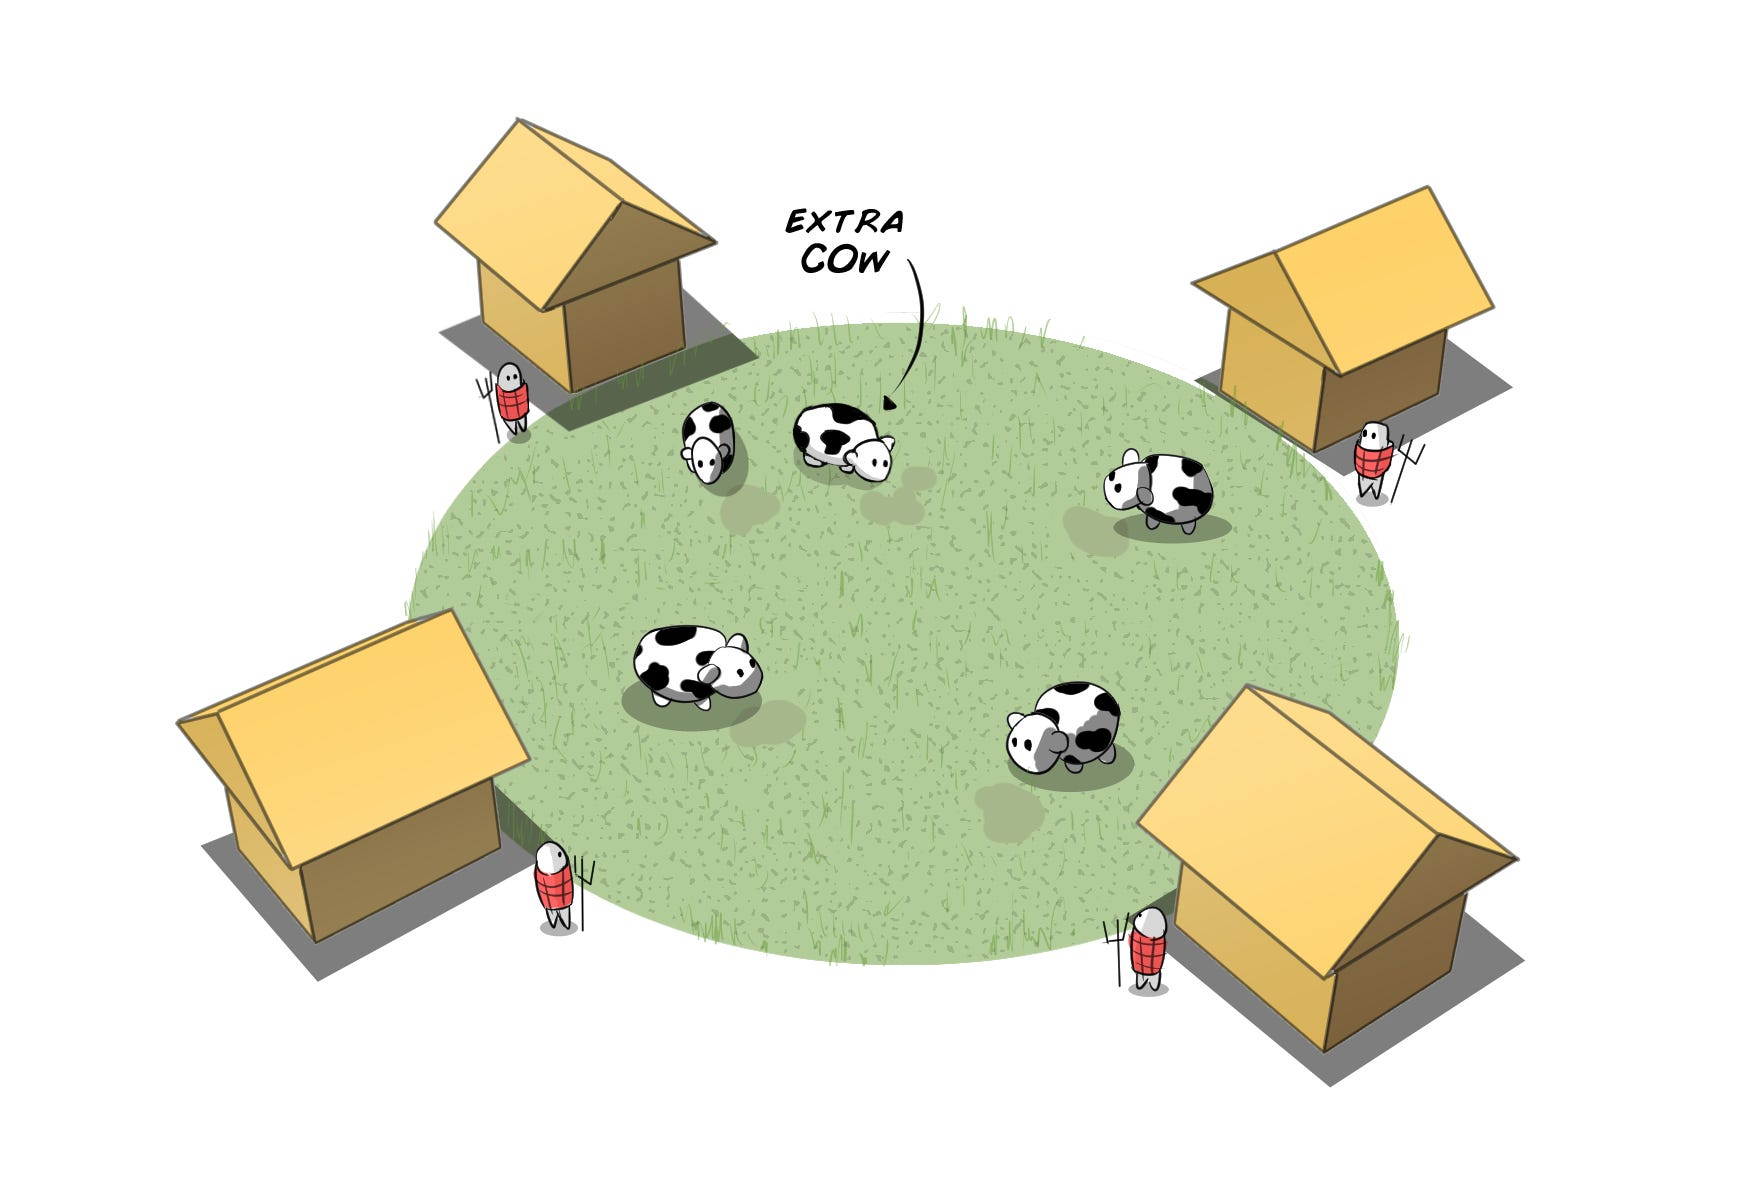
\includegraphics[alt={tragedy of commons classic},height=1.6in]{tragedy-of-commons-classic.jpg}



Modern instantiation: air pollution.

\begin{itemize}
\item Air is a common good.
\item Each country affects every other country's air.
\item A country can reduce polution at a cost of -10 (to implement reduction technology, reduced economic output, etc.).
\item A country can continue to polute at a cost of -5 (added health costs, etc), but this also adds a -1 cost to all other countries.
\end{itemize}

So, if there are 100 countries and each continues to pollute, the total utility for each country is -104 -- far greater than the -10 for reducing pollution.  This is a version of The Prisoner's Dilemma.
\section{Nash Equilibria}
\label{sec:orgb4dac2d}


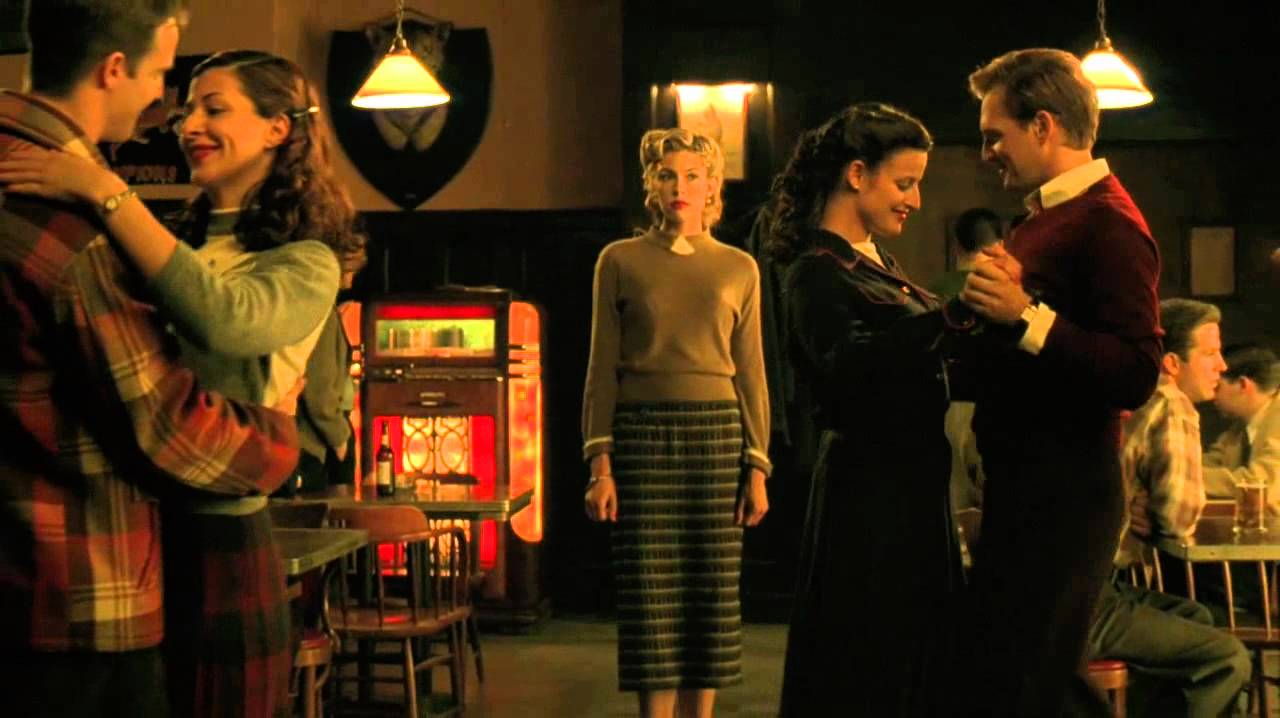
\includegraphics[alt={beautiful mind bar scene},height=1.6in]{beautiful-mind-bar-scene.jpg}


\href{https://www.youtube.com/watch?v=QzwcGkfEra4}{https://www.youtube.com/watch?v=QzwcGkfEra4}




A strategy profile is a \textbf{Nash equilibrium} if no player could unilaterally change their strategy and as a consequence receive a higher payoff, under the assumption that the other players
stayed with their strategy choices.

\begin{itemize}
\item In a Nash equilibrium, every player is simultaneously playing a best response to the choices of their counterparts.
\item A Nash equilibrium represents a stable point in a game: stable in the sense that there is no rational incentive for any player to deviate.
\item However, Nash equilibria are local stable points: as we will see, a game may contain
\end{itemize}
multiple Nash equilibria.
\section{Finding Nash Equilibria}
\label{sec:orge67e109}

Let's find the Nash equlibria in the Prisoner's Dilemma.

\begin{itemize}
\item First, find the best reponses of the row player to each strategy of the column player (boxed):
\end{itemize}


\begin{tabular}{|c|c|c|}\hline
  & C              & D         \\\hline
C & -1, -1         & -5, 0 \\\hline
D & \boxed{0}, -5  & \boxed{-3}, -3 \\\hline
\end{tabular}


\begin{itemize}
\item Then find the best responses of the column player to each strategy of the column player (circled):
\end{itemize}


\begin{tabular}{|c|c|c|}\hline
  & C              & D         \\\hline
C & -1, -1         & -5, \circled{0} \\\hline
D & \boxed{0}, -5  & \boxed{-3}, \circled{-3} \\\hline
\end{tabular}


The Nash equilibria are the cases where both players' best responses coincide, here \((D, D)\).

This is sometimes called a "no regret" decision -- couldn't have done better given what other players did.
\section{Coordination and Competition: Battle of the Sexes (MAS 3.2.3)}
\label{sec:org23c3889}

A husband and wife wish to go to the movies, and they can select among two movies:
"Lethal Weapon (LW)" and "Wondrous Love (WL)."

\begin{itemize}
\item They much prefer to go together rather than to separate movies, but
\item the wife (player 1) prefers LW, the husband (player 2) prefers WL.
\end{itemize}


\begin{tabular}{|c|c|c|}\hline
   & LW     & WL         \\\hline
LW & 2, 1  & 0, 0 \\\hline
WL & 0, 0  & 1, 2 \\\hline
\end{tabular}


This is like a common-payoff game where both players get the same reward when they do the same thing, but each player has different payoffs when they coordinate.
\section{Multiple Nash Equilibria}
\label{sec:org4b7b7d5}

Now lets find the Nash equilibria for the Battle of t he Sexes game.

\begin{itemize}
\item First, find the best reponses of the row player to each strategy of the column player (boxed):
\end{itemize}


\begin{tabular}{|c|c|c|}\hline
   & LW     & WL         \\\hline
LW & \boxed{2}, 1  & 0, 0 \\\hline
WL & 0, 0  & \boxed{1}, 2 \\\hline
\end{tabular}


\begin{itemize}
\item Then find the best responses of the column player to each strategy of the column player (circled):
\end{itemize}


\begin{tabular}{|c|c|c|}\hline
   & LW     & WL         \\\hline
LW & \boxed{2}, \circled{1}  & 0, 0 \\\hline
WL & 0, 0  & \boxed{1}, \circled{2} \\\hline
\end{tabular}


Here we see that the only best responses for both players are also both Nash equilibria.
\section{Iterated Prisoner's Dilemma (IPD)}
\label{sec:org810064a}

The simplest kind of multiple-move game is the repeated game (also called an \textbf{iterated game}), in which players repeatedly play rounds of a single-move game, called the \textbf{stage game}.

\begin{itemize}
\item A strategy in a repeated game specifies an action choice for each player at each time step for every possible history of previous choices of players.
\item In a finite game you essentially end up with a single game repeated \(n\) times, because if you know the last game is the last, then you simply play the single-game dominant strategy.  This leads to playing the same for the \$n-1\$st game, and so on.
\item In an infinite game you don't know when it ends, so strategy changes.  We can represent infinite strategies with finite state machines:
\end{itemize}


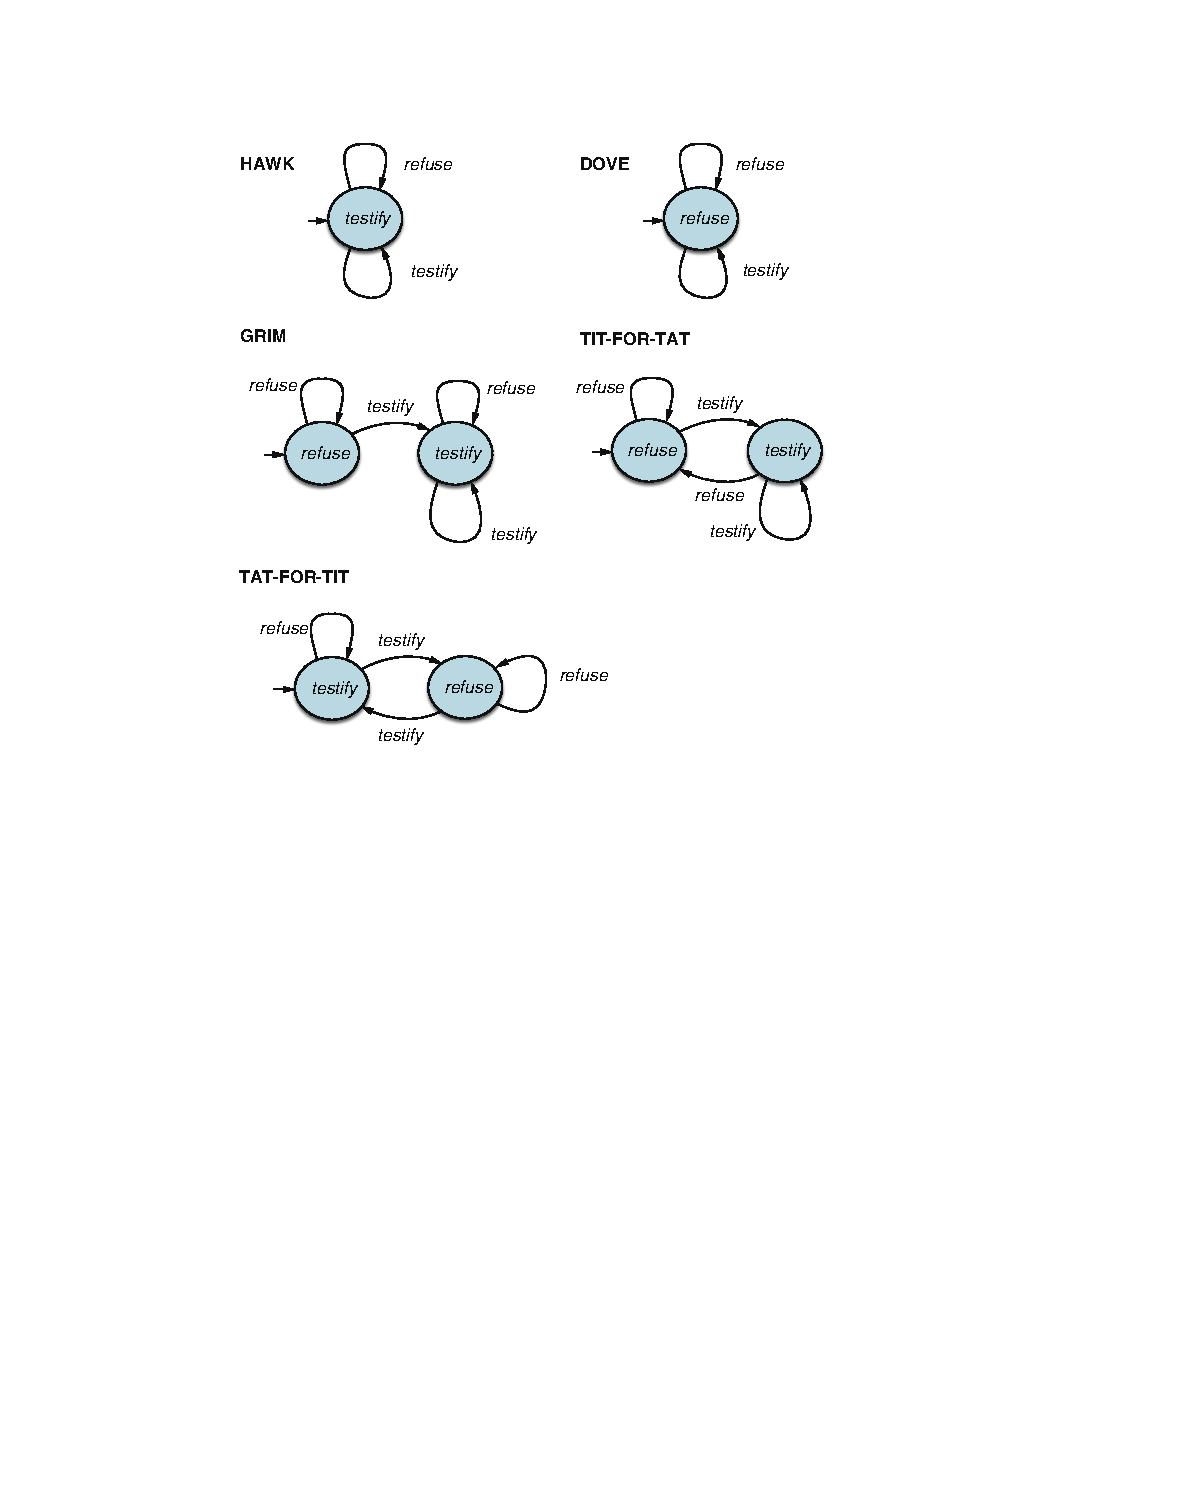
\includegraphics[alt={aima fig 18_03 ipd fsms},height=1.6in]{aima-fig-18_03-ipd-fsms.pdf}



Note that AIMA uses \(refuse\) for \(confess/cooperate\) and \(testify\) for \(deny/defect\).
\section{Axelrod's IPD Tournaments}
\label{sec:org1000b9a}





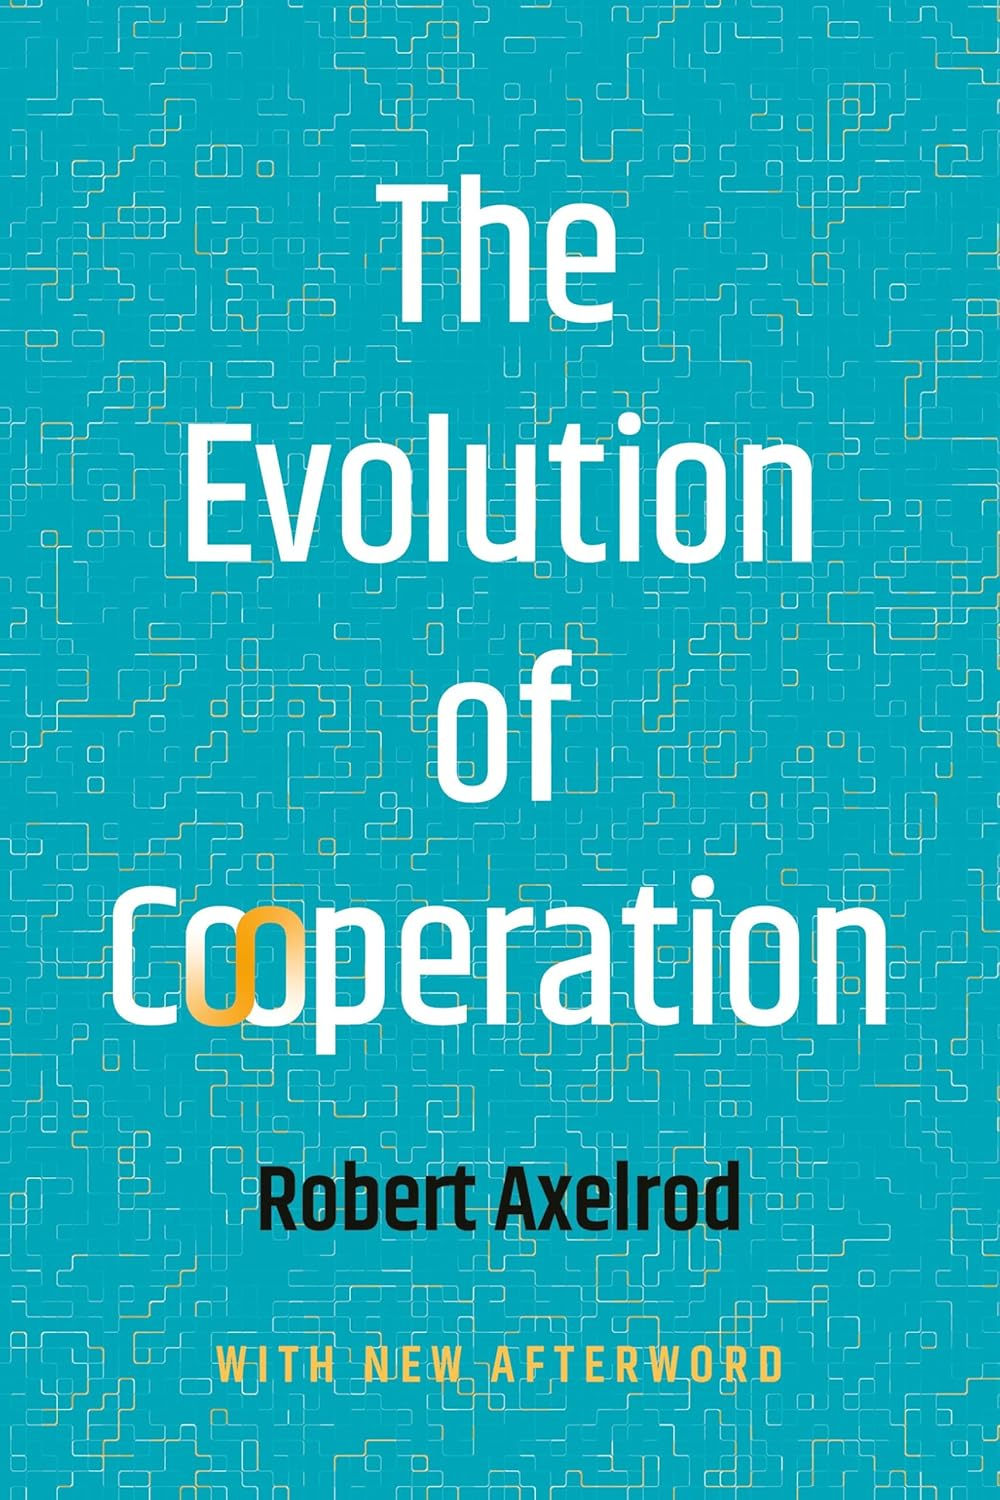
\includegraphics[alt={axelrod evolution of cooperation book},height=3.2in]{axelrod-evolution-of-cooperation-book.jpg}






In the 1980s, Robert Axelrod organized a series of computer tournaments in which computer programs submitted by contestants implemented any strategy of their choosing.  Suprising key findings:

\begin{itemize}
\item Tit for tat was the winning strategy.
\item Starting out cooperate is better.
\item Adding forgiveness helps.
\end{itemize}

Knight, et. al. [\textsuperscript{knight2025reviving}] recently reproduced these results, confirming that "TFT prevails, and successful play tends to be cooperative, responsive to defection, and willing to forgive."

{[}\textsuperscript{knight2025reviving}]: \url{https://arxiv.org/abs/2510.15438}
\section{Closing Thoughts: Rational Altruism}
\label{sec:org0988bb2}





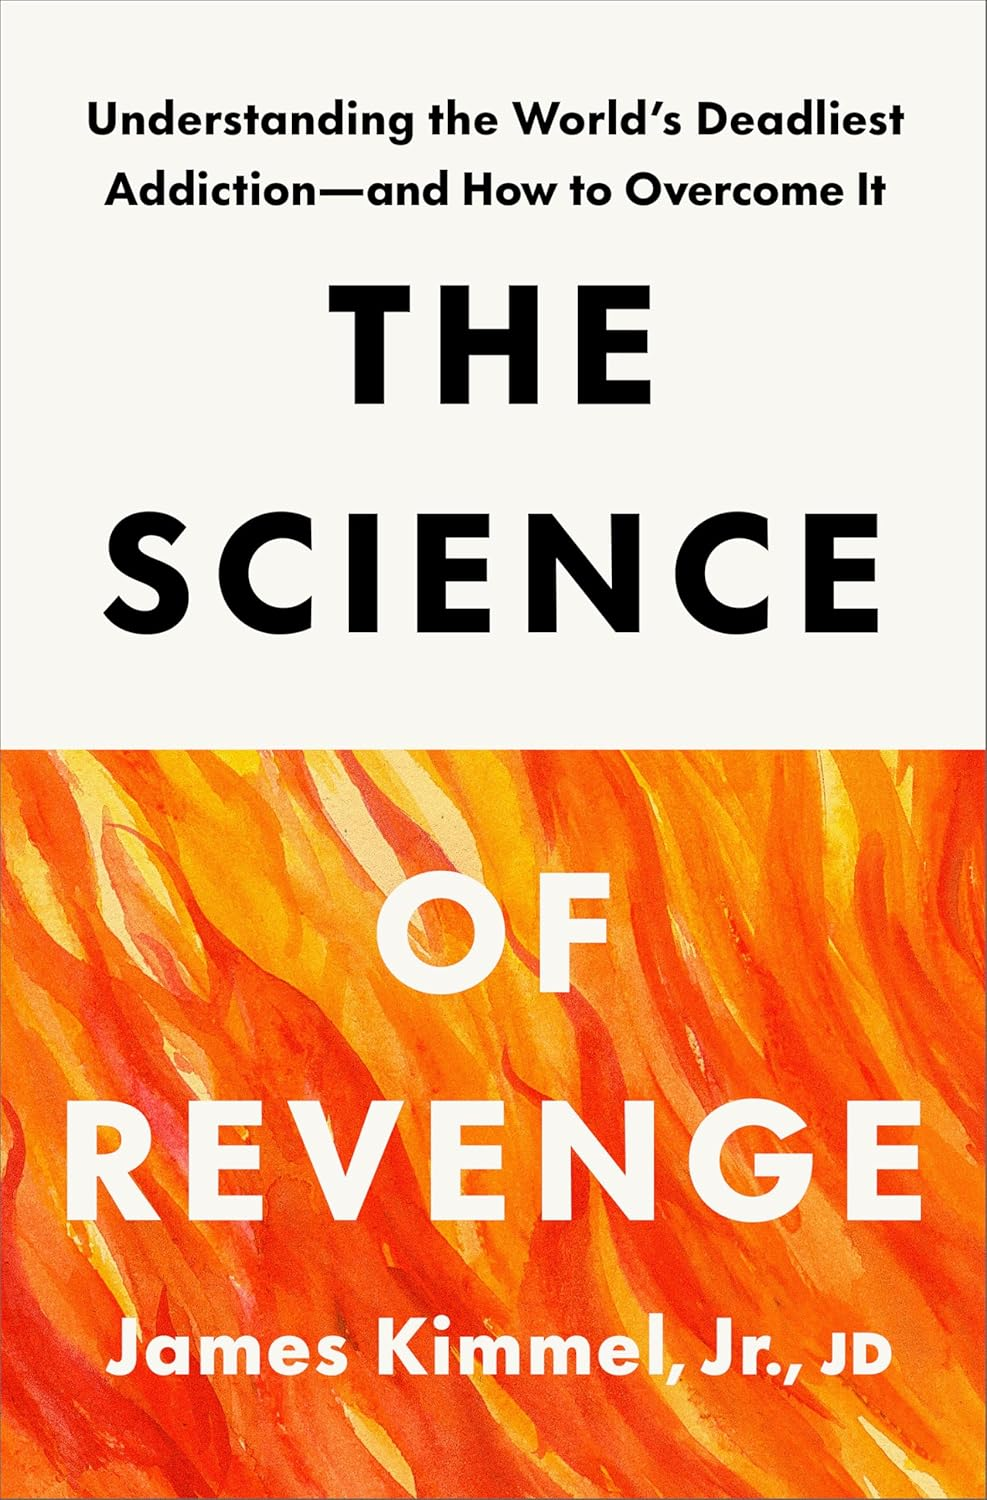
\includegraphics[alt={kimmel science of revenge book},height=3.2in]{kimmel-science-of-revenge-book.jpg}






The lesson of The Prisoner's Dilemma is that individually rational action often leads not just to lower total \textbf{social} utility, but lower \textbf{indivdual} utility over the long run.

\begin{itemize}
\item Previously we saw that if an agent's utility function aligns with the external performance measure of its task environment, then maximizing its utility maximizes its performance.
\item How do we get global utility into local utility functions?
\end{itemize}

There is exciting research in neuroscience that suggests that social good and individual utility are aligned.

\begin{itemize}
\item Revenge triggers the same dopamine reponse as addiction.
\item Forgiveness cuts this cycle.
\end{itemize}

Perhaps there is a link between the results of Axelrod's IPD tournaments and neurobiology.




{[}\textsuperscript{kimmel2025science}]: \url{https://www.amazon.com/Science-Revenge-Understanding-Deadliest-Addiction/dp/0593796519}
\section{Lessons from Animals}
\label{sec:orgb779397}






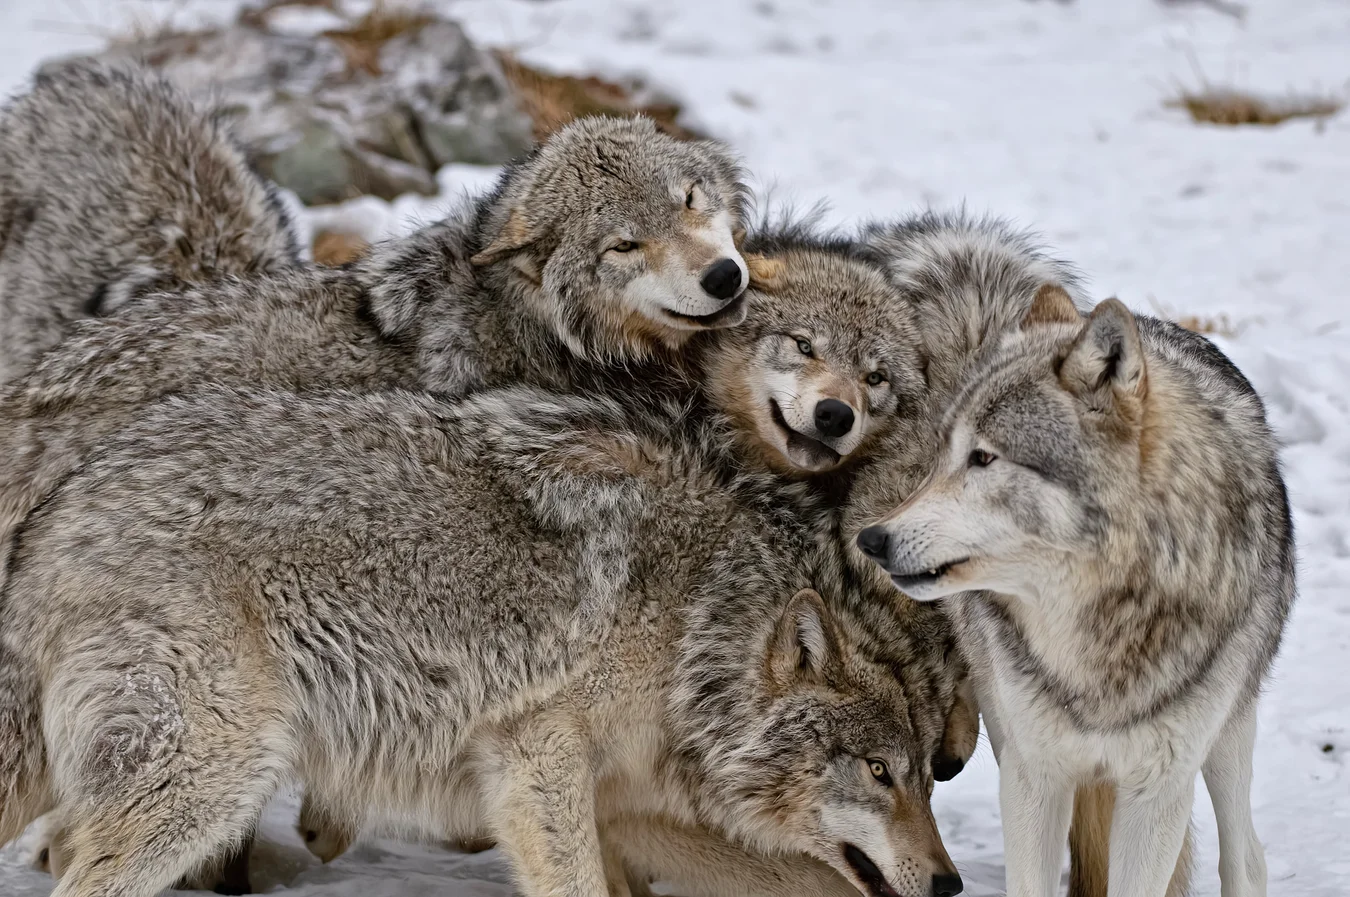
\includegraphics[alt={wolf pack},height=1.6in]{wolf-pack.png}


\vspace{.1in}


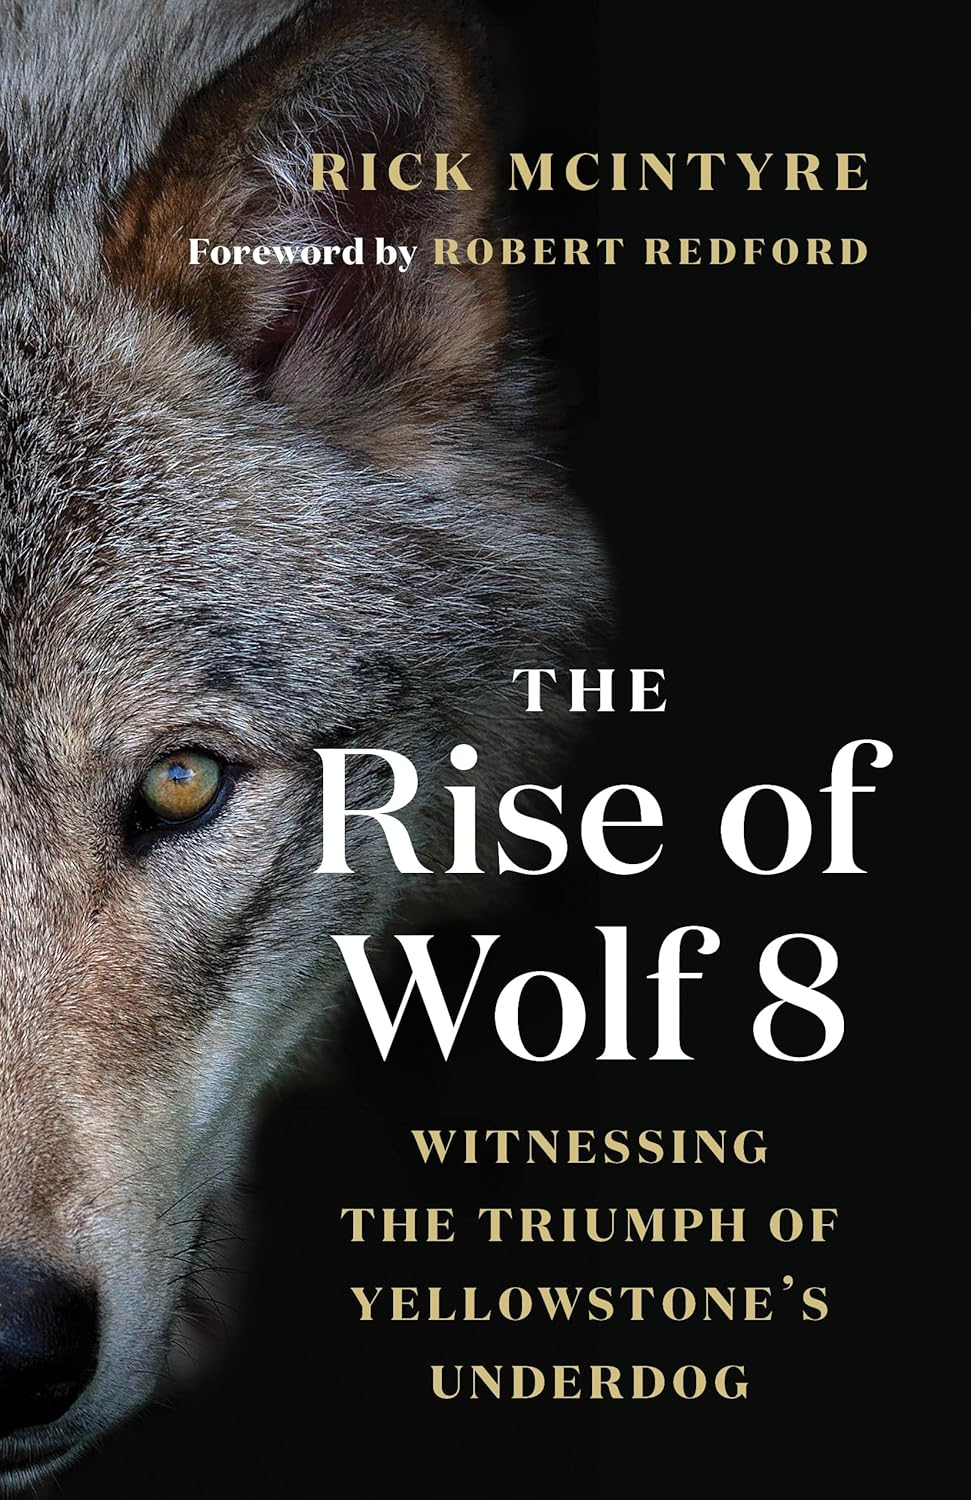
\includegraphics[alt={rise of wolf 8 book},height=2.0in]{rise-of-wolf-8-book.jpg}







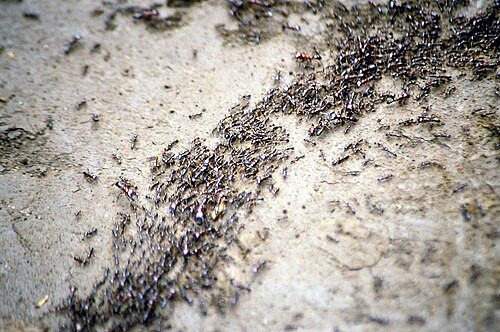
\includegraphics[alt={Safari_ants},height=1.2in]{Safari_ants.jpg}


\vspace{.1in}


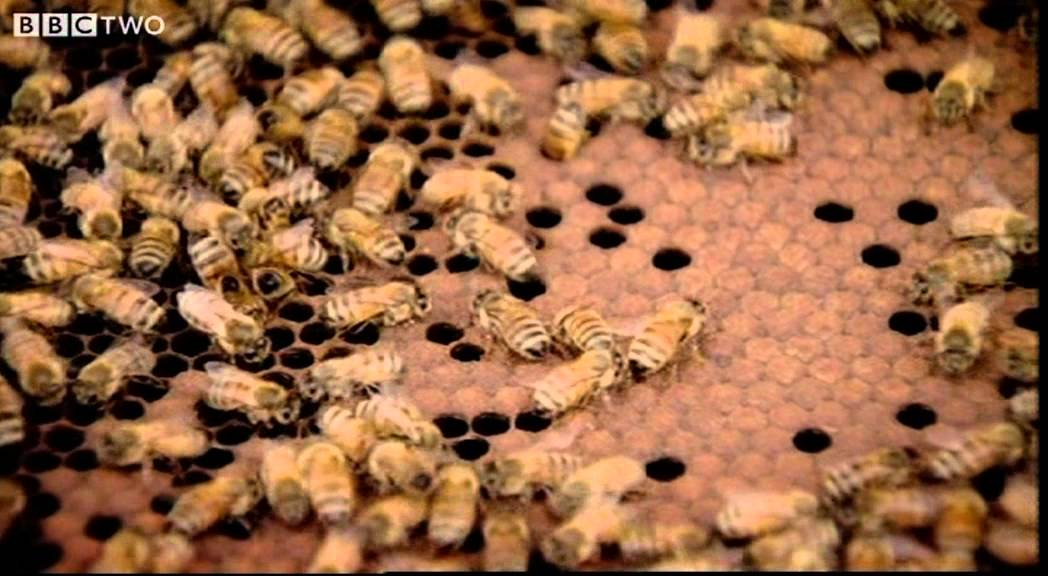
\includegraphics[alt={bees honeycomb},height=1.2in]{bees-honeycomb.jpg}


\href{https://www.youtube.com/watch?v=F5rWmGe0HBI}{https://www.youtube.com/watch?v=F5rWmGe0HBI}
\section{Humans are Complicated Animals}
\label{sec:orgfc0a2ca}

Humans are complicated -- and often amusing -- animals.  The Prisoner's Dilemma often occurs naturally, and sometimes artificially:



\includegraphics[alt={bachelor pad prisoners dilemma.},height=2.0in]{bachelor-pad-prisoners-dilemma.jpeg}


\href{https://www.youtube.com/watch?v=p1oyuqLFiXg}{https://www.youtube.com/watch?v=p1oyuqLFiXg} -- 1:06:30
\end{document}
